\section{Heap}\label{sec:heap}

Ein \textbf{Heap} (\textit{Halde}) ist eine Datenstruktur, die nach \textit{Ottmann und Widmayer} wie folgt definiert ist:

\blockquote[{\cite[106]{OW17b}}]{
Eine Folge $F = K_1, k_2, \ldots,k_N$ von Schlüsseln nennen wir einen Heap, wenn $k_i \leq k_{\lfloor \frac{i}{2} \rfloor}$ für $2 \leq i \leq N$ gilt. Anders ausgedrückt: $k_i \geq k_{2i}$ und $k_i \geq k_{2i+1}$, sofern $2i \leq N$ bzw. $2i + 1 \leq N$.
}

\noindent
Die Folge $12, 9, 6, 4, 8, 5, 1, 2$ ist ein Heap (s. Tabelle~\ref{tab:heap}).
Es gilt:

\begin{enumerate}
    \item $12_1 \geq 9_2 \land 12_1 \geq 6_3$
    \item $9_2 \geq 4_4 \land 9_2 \geq 8_5$
    \item $6_3 \geq 5_6 \land 6_3 \geq 1_7$
    \item $4_4 \geq 2_8$
\end{enumerate}


\setlength{\tabcolsep}{1.5em}
\renewcommand{\arraystretch}{1.5}%
\begin{table} %[hbtp]
    \centering
    \begin{tabular}{|l | c | c | c| c| c | c| c | c|}
        \hline
        $i$ & $1$ &  $2$ &  $3$ &  $4$ &  $5$ &  $6$ &  $7$ &  $8$  \\
        \hline
        $k_i$ & $12$ &  $9$ &  $6$ &  $4$ &  $8$ &  $5$ &  $1$ &  $2$  \\
        \hline
    \end{tabular}
    \caption{Beispiel für einen Heap.}
    \label{tab:heap}
\end{table}

\noindent
Insbesondere liefert die Beziehung $k_i \geq k_{2i}$ und $k_i \geq k_{2i+1}$ eine einfache Vorschrift für die grafische Darstellung eines Heaps als \textbf{links-vollständigen} binären Baumes\footnote{
alle Ebenen bis auf die letzte sind voll besetzt; auf der letzten Ebene sitzen die Knoten so weit links wie möglich (vgl.~\cite[154]{GD18d})
} (s. Abbildung~\ref{fig:heaptree}):

\blockquote[{\cite[107]{OW17b}}]{
   Ein Binärbaum ist ein Heap, wenn der Schlüssel jedes Knotens mindestens so groß ist wie die Schlüssel seiner beiden Söhne (falls es diese gibt).
}

\begin{figure}
    \begin{center}
        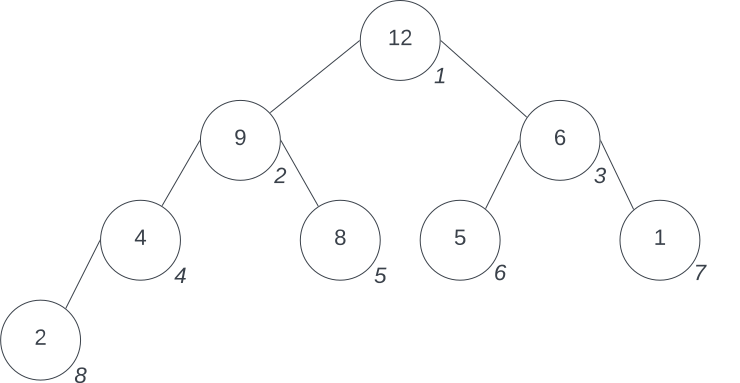
\includegraphics[scale=0.4]{chapters/Datenstrukturen und Algorithmen/img/heaptree}
        \caption{Der Heap  $12, 9, 6, 4, 8, 5, 1, 2$ als binärer Baum (Quelle: eigene)}
        \label{fig:heaptree}
    \end{center}
\end{figure}

\subsection{Min-Heap / Max-Heap}
Man kann zwischen \code{Min-Heaps} und \code{Max-Heaps} unterscheiden.\\
Bisherige Betrachtungen bezogen sich auf einen \code{Max-Heap} - die Schlüssel der direkten Nachfolger eines Knotens sind kleiner-gleich des Schlüssels des Vaterknotens.\\
Bei \textbf{Min-Heaps} ist die Bedingung, dass die Schlüssel der direkten Nachfolger eines Knotens größer-gleich des Schlüssels des Vaterknotens sind.\\

\subsection{Algorithmen für Heaps}
Sind nach dem Einfügen eines Schlüssels die Heap-Bedingungen verletzt, müssen diese wiederhergestellt werden.

\subsubsection{swim}

\textbf{Bottom-up reheapify (swim)} (vgl.~\cite[315]{SW11}) kann angewendet werden, um einen neu einzufügenden Schlüssel an seine richtige Position in dem Heap zu bewegen.

\noindent
In dem o.a. Beispiel soll ein neuer Schlüssel $20$ eingefügt werden.\\
Entsprechend der Implementierung als Folge wird der Schlüssel an das Ende angehangen: $12, 9, 6, 4, 8, 5, 1, 2, 20$\\

\noindent
Die Heap-Bedingung für $k_4$ ist nun verletzt wegen $4_4 \geq 2_8 \nand 4_4 \ngeq 20_9$.
Um die Heap-Bedingung wieder herzustellen, muss der Schlüssel an seine richtige Position wandern.\\
Hierzu wird er sukzessive mit seinem direkten Vorgänger (dem Vaterknoten $k_{\lfloor \frac{i}{2} \rfloor}$) ausgetauscht, bis $k_{\lfloor \frac{i}{2} \rfloor}$ größer $k_9$ ist oder die Wurzel des Heaps erreicht ist.\\
Anwendung dieses Verfahrens liefert die Folge $20, 12, 6, 9, 8, 5, 1, 2, 4$  (s. Abbildung~\ref{fig:swim}).

\begin{figure}
    \begin{center}
        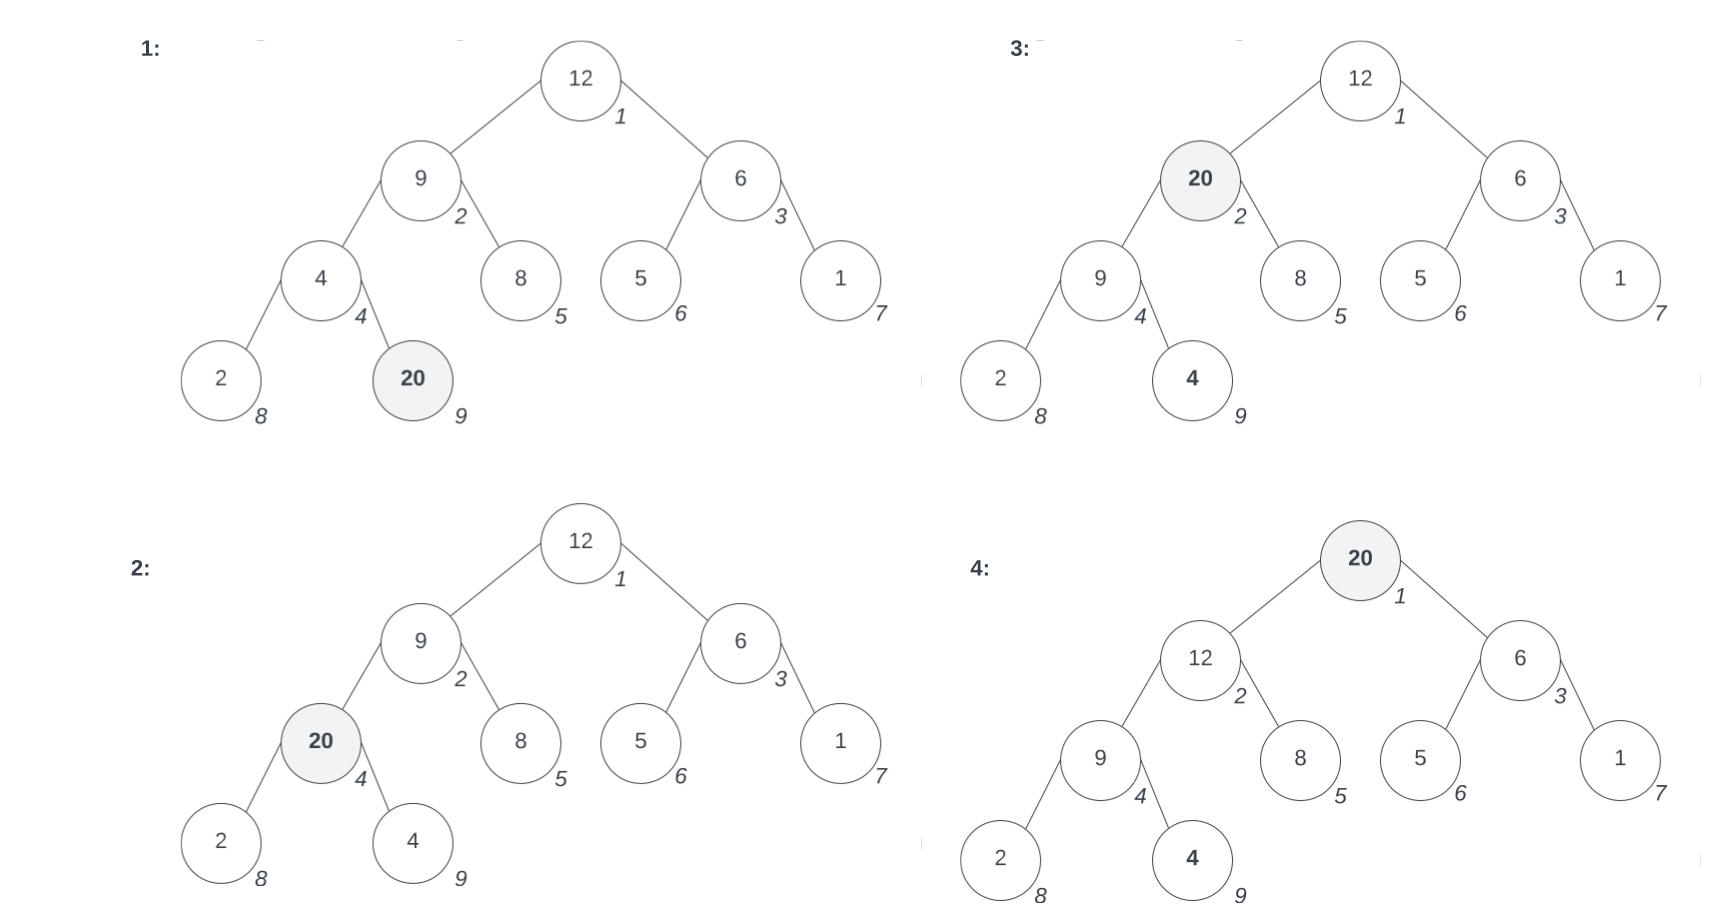
\includegraphics[scale=0.25]{chapters/Datenstrukturen und Algorithmen/img/swim}
        \caption{Wiederherstellung der Heap-Bedingungen nach Einfügen des Schlüssels $20$ durch \textbf{bottom-up reheapify}(Quelle: eigene)}
        \label{fig:swim}
    \end{center}
\end{figure}

\subsubsection{sink}
Sollte ein Schlüssel \textit{kleiner} als seine direkten Nachfolger sein, kann \textbf{top-down reheapify (sink)}\footnote{\textit{sift down} (\textit{versickern}) bei \textit{Ottmann und Widmayer} (vgl.~\cite[107 f.]{OW17b})} angewendet werden.\\

\noindent
Hierbei tauscht der Schlüssel die Position mit dem jeweils \textit{größeren} seiner direkten Nachfolger, bis die Heap-Bedingungen wieder hergestellt sind (s. Abbildung~\ref{fig:sink}).\\


\begin{figure}
    \begin{center}
        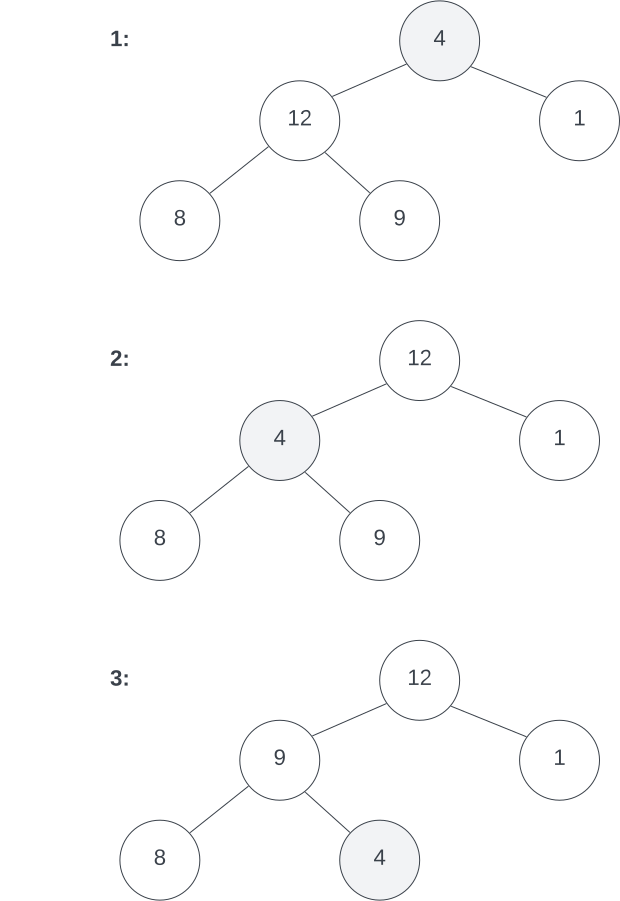
\includegraphics[scale=0.35]{chapters/Datenstrukturen und Algorithmen/img/sink}
        \caption{Herstellung der Heap-Bedingungen für die Folge $4, 12, 1, 8, 9$ mittels \textbf{top-down reheapify} (Quelle: eigene)}
        \label{fig:sink}
    \end{center}
\end{figure}


